\documentclass[12pt]{article}
\usepackage[T1]{fontenc}
%\usepackage[latin9]{inputenc}
\usepackage[utf8]{inputenc}
\usepackage[english]{babel}
\usepackage{amsmath}
\usepackage{amsfonts}
\usepackage{amssymb}
\usepackage{setspace}
\usepackage{rotating}
\usepackage{graphics}
\usepackage[round]{natbib}
\usepackage{graphicx}
\usepackage{float} 				%allows you to float images
\usepackage{latexsym}
\usepackage{bbding}
\usepackage {moresize}
\usepackage{bbding}
\usepackage{blindtext}
\usepackage{hhline}
\usepackage{tikz}
\usetikzlibrary{shapes,backgrounds}
\usepackage{pgfplots}
\usetikzlibrary{arrows}
\usepackage{enumitem}
\doublespacing
\usepackage{geometry}
\usepackage{amsthm}
\usepackage{color}
\usepackage{array,multirow}
\usepackage{subcaption}
\usepackage{pst-plot}
	\psset{xunit=15mm}
\geometry{verbose,tmargin=1in,bmargin=1in,lmargin=1in,rmargin=1in}
\setlength{\parskip}{\bigskipamount}
\setlength{\parindent}{0pt}

\newenvironment{problem}[2][Problem]{\begin{trivlist}
\item[\hskip \labelsep {\bfseries #1}\hskip \labelsep {\bfseries #2.}]}{\end{trivlist}}

\title{Problem Set 3 \thanks{Problem list - 3.4.4, 3.5.14, 3.5.32, 3.6.2, 3.6.10}}
\author{Ian McGroarty \\
	Course Number: 625.603}
\date{February 21, 2019}

\begin{document}

\maketitle

\begin{problem}{3.4.4} Remission time is $f_Y(y) = \frac{1}{9}y^2$, $0 \leq y \leq 3$. What is the probability the patients malaria lasts longer than one year?

\textbf{Solution} The probability that a malaria patients remisssion lasts longer than one year is 0.963, or 96.3\%.   
\begin{align*}
F_Y(y) &= \int f_Y(y)dy  && \text{Def 3.4.3 pg 135} \\
&= \int \frac{1}{9} y^2 dy \\
&= \frac{1}{27}y^3 && \text{This is the cdf.} \\
P(Y>s) &= 1-F_Y(s) && \text{Theorem 3.4.2(a) pg 135} \\
P(Y>1) &= 1 - \frac{1}{27}(1^3) \\
	&= \frac{26}{27} \\
P(Y>1) &= 0.963
\end{align*}
\end{problem}

\begin{problem}{3.5.14} 15 observations are chosen at random from pdf $f_Y(y) = 3y^2, \ 0 \leq y \leq 1$. Let X denote the number that lie in the interval $(\frac{1}{2},1)$. Find $E(X)$. 

\textbf{Solution} 
First, we must determine the probability that any given obseravtion is in the interval $(\frac{1}{2},1)$. To do this we evaluate the area under the pdf on the given interval. 
\begin{align*}
P(r<Y\leq s) &= F_Y(s) - F_Y(r) && \text{Theorem 3.4.2 pg 135} \\
&= \Big|_{\frac{1}{2}}^1 F_Y && \text{Interested in the interval 1/2 to 1} \\
&= \int_{\frac{1}{2}}^1 f_Y(y) dy && \text{Def 3.4.3 pg 135} \\
&= \int_{\frac{1}{2}}^1 3y^2 dy \\
&= y^3  \Big|_{\frac{1}{2}}^1  \\
&= 1^3 - (\frac{1}{2})^3  \\
&= \frac{7}{8} \\
\end{align*}
Since the events of X are mutually exclusive, axiom 3 (pg 26) apples. $E(X)=15(7/8)=105/8$. 
\end{problem}

\begin{problem}{3.5.32} Box with height 5in. and base YxY inches. Where Y is a random variable with $pdf$ $f_Y(y)=6y(1-y), \ 0 < y < 1$. Find the expected volume of the box. 
\\
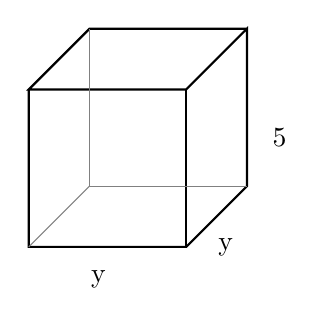
\begin{tikzpicture}
  \draw[thick](2,2,0)--(0,2,0)--(0,2,2)--(2,2,2)--(2,2,0)--(2,0,0)--(2,0,2)--(0,0,2)--(0,2,2);
  \draw[thick](2,2,2)--(2,0,2);
  \draw[gray](2,0,0)--(0,0,0)--(0,2,0);
  \draw[gray](0,0,0)--(0,0,2);
  \draw(2.5,0,2) node{y};
  \draw(1,2,1) node{};
  \draw(2.8,1,1) node{5};
  \draw(0.5,-0.8,1) node{y};
  \draw(0,1,1) node{};
  \draw(1,1,0) node{};
\end{tikzpicture}


\textbf{Solution} The box has an expected area of 1.5 inches. \\
The area of the box is A=$5(Y^2)$ Let area be defined as g(Y), a continuous funtion. Then: 
\begin{align*} 
E[g(Y)] &= \int g(y) \cdot f_Y(y) dy && \text{Theorem 3.5.3 pg 148} \\
&= \int_0^1 (5y^2)\cdot 6y(1-y) dy && \text{Interested in interval 0 to 1}\\
&= 30\int_0^1 y^3 -y^4 dy \\
&= 30 ( \frac{y^4}{4} - \frac{y^5}{5} \Big|_0^1 ) \\
&= \frac{30}{4} - {30}{5} \\
&= \frac{30}{20} = \text{ 1.5 inches.}
\end{align*}
\end{problem}

\begin{problem}{3.6.2} Find the variance of Y if: 
$$
f_Y(y) = \left\{
        \begin{array}{ll}
            \frac{3}{4}, & \quad 0 \leq y \leq 1 \\
            \frac{1}{4}, & \quad 2 \leq y \leq 3 \\
		0,  & \quad \text{elsewhere}
        \end{array}
    \right.
$$
\textbf{Solution} $Var(Y) = \frac{5}{8}$ or 0.833. 
\begin{align*} 
E(Y) = \mu &= \int_0^1 y(\frac{3}{4}) dy + \int_2^3y(\frac{1}{4})dy && \text{First need to find Expected value of y}\\
&= (\frac{3}{8})y^2 \Big|_0^1 + (\frac{1}{8})y^2 \Big|_2^3  \\
&= (\frac{3}{8}) + (\frac{9}{8} - \frac{4}{8}) = 1 \\
E(Y^2) = \mu &= \int_0^1 y^2(\frac{3}{4}) dy + \int_2^3y^2(\frac{1}{4})dy && \text{Now need to find Expected value of $y^2$}\\
&= (\frac{3}{12})y^3 \Big|_0^1 + (\frac{1}{12})y^3 \Big|_2^3 \\
&= (\frac{3}{12}) + (\frac{27}{12}-\frac{8}{12}) = \frac{22}{12}\\
Var(Y) & = \sigma^2 = E(Y^2)-\mu^2 && \text{Theorem 3.6.1 pg 155} \\
&= \frac{22}{12} - \frac{12}{12} = \frac{10}{12}
\end{align*}
\end{problem} 

\begin{problem}{3.6.10}Let Y be a random variabe whose pdf is given by $f_Y(y) = 5y^4, \ 0 \leq y \leq 1$. Find Var(Y). 

\textbf{Solution} $Var(Y) = \frac{5}{32} $ or 0.1562
\begin{align*}
E(Y) = \mu &= \int_0^1 y \cdot 5y^4 dy  && \text{First need to find Expected value of y}\\
&= \int_0^1 5y^5 dy\\
&= (\frac{5}{6})y^6 \Big|_0^1 = \frac{5}{6}\\
E(Y^2) = \mu_2 &= \int_0^1 y^2 \cdot 5y^4 dy && \text{Now to find expected value of $y^2$} \\
&= \int_0^1 5y^6 dy \\
&= (\frac{5}{7})y^7 \Big|_0^1 = \frac{5}{7} \\
Var(Y)  = \sigma^2 &= E(Y^2)-E(Y)^2 = \mu_2 - \mu^2  && \text{Theorem 3.6.1 pg 155} \\
&= \frac{5}{7} - (\frac{5}{6})^2 = \frac{5}{252}
\end{align*}
\end{problem}


\end{document}